\documentclass[PlasmaNotes.tex]{subfiles}
\begin{document}
\setcounter{section}{2}
\section{Week 3. Fluid description of plasmas, with Paolo Ricci}
\subsection{From Vlasov to two-fluid}

\begin{itemize}
\item We'll turn the computationally expensive kinetic model into a simple fluid model (can be solved with partial differential function)
\item We'll derive fluid quantities (pressure, etc) from distribution functions
\item We'll take a moment for moments of the kinetic equation
\item We'll apply the continuity equation (conservation of mass etc)
\item ... and we'll get the two fluid model!
\end{itemize}

\subsubsection{Fluid quantities from the distribution function}
In the fluid model we only really look at quantities that depend on position. This means we'll have to integrate out all velocity dependence.

Number density - the integral of distribution function over all velocities. Simple. We just care about the density \emph{at a location}.
\[n_s(r,t) = \int{dv f_s(r, v, t)} \]

For any function $g(r, v)$, it's average value is the integral of the function weighted by distribution function, normalized by dividing the integral by the number density of the species.
\[ \avg{g(r)} = \oneover{n_s} \int{g(r, v) f_s(r,v, t) d_v} f \]

Examples:
\begin{itemize}
\item Average fluid velocity, $g(v) = v$
\[ u_s(r,t) = \oneover{n_s} \int{v f_s(r,v,t) dv} \]
\item Average kinetic energy density, $g(v) = \oneover{2} m_s v^2$
\[ w_s(r,t) = \oneover{n_s} \int{ \oneover{2} m_s v^2 f_s(r,v,t) dv} \]
\item Pressure \textbf{tensor} (as pressure may depend on direction), $g(v) = m_s (\v{v} -\v{u_s})(\v{v} -\v{u_s})$ - a tensor (dyadic) quantity)
\[ \hat{P} = \int m_s (\v{v} -\v{u_s}) (\v{v} -\v{u_s}) f_s(r,v,t) \]
\end{itemize}

\subsubsection{Examples of fluid averaged quantities}
\begin{enumerate}
\item Beam density. Distribution function with uniform spread in $1D$ positions and a delta function dependence on velocity (only one velocity in the whole beam

\[ f = n_0 \delta(\v{v} - \v{v_0}) \]

The density ends up being just $n_0$ because of the Dirac delta velocity dependence.

The fluid velocity is just the velocity of the particles, as the delta function times velocity gives us just the particle velocity upon integrating out.

The kinetic energy density is just $m v_0^2/2$, obviously.

The pressure tensor ends up as zero! Both the vector quantities end up being zero as $\v{v} = \v{v_0}$. Reasonable. If everything's moving at the same velocity there's not going to be anything pushing anything else.

\item Maxwellian velocity distribution with uniform position distribution
\[ f = n_0 \Big( \frac{1}{2 \pi v_{th}^2} \Big)^{3/2} \exp{\frac{-(\v{v}-\v{v_0})^2}{2 v_{th}^2}} \]

Note that the lecture had a version with masses. This was corrected in the errata - I suppose because we're working in position-velocity phase space instead of position-momentum phase space.

Number density is just $n_0$, as the velocity distribution is normalized to one anyway.

Average fluid velocity - gaussian average value $v_0$. 

Average kinetic energy density: kinetic energy from average velocity plus $\frac{3}{2} k_b T$ (thermal velocity)

Pressure tensor is a diagonal matrix.
\[\hat{P} = 
\begin{pmatrix}
n_0 T & 0 & 0 \\
0 & n_0 T & 0 \\
0 & 0 & n_0 T
\end{pmatrix} \]

Note that in the errata, $n_0 K_B T$ (from the lecture) was corrected to $n_0 T$, as in this course temperatures are defined thermodynamically, through energy, including the Boltzmann constant.

\end{enumerate}

\subsubsection{The moments of the kinetic equation}

We take the Boltzmann equation:

\[ \pd{f_s}{t} + \dotproduct{v}{\pd{f_s}{r}} + \frac{q_s}{m_s}\dotproduct{(E+\crossproduct{v}{B})}{\pd{f_s}{v}} = \Big(\pd{f_s}{t}\Big)_c \]

Shift the collision term to the left side and denote the whole thing, which is now equal to zero for all positions, times and velocities (I'll denote this as $BOLT$):

\[BOLT = \pd{f_s}{t} + \dotproduct{v}{\pd{f_s}{r}} + \frac{q_s}{m_s}\dotproduct{(E+\crossproduct{v}{B})}{\pd{f_s}{v}} - \Big(\pd{f_s}{t}\Big)_c = 0  \]
And take averages - `moments' - of that by integrating $BOLT$ with a weight $g$. This will give us the following equations:
\begin{itemize}
\item Continuity for $g=1$
\item Momentum for $g=mv$
\item Energy for $g=mv^2/2$
\end{itemize}
The continuity equation will be done here. The rest are, in true physics tradition, easy to derive and as such are left to the reader.

\subsubsection{The continuity equation}

\[ \int{BOLT dv} = \int{ \Big( \pd{f_s}{t} + \dotproduct{v}{\pd{f_s}{r}} + \frac{q_s}{m_s}\dotproduct{(E+\crossproduct{v}{B})}{\pd{f_s}{v}} - \Big(\pd{f_s}{t}\Big)_c\Big) dv} = 0 \]

\begin{itemize}
\item The first term ends up as just the time derivative of average number density
\[ \int{\pd{f_s}{t} dv} = \pd{}{t} \int{f_s dv} = \pd{n_s}{t} \]
\item The second term is the time derivative of average fluid velocity times average number density
\[ \int{\dotproduct{v}{\pd{f_s}{r}} dv} = \pd{}{r} \int{v f_s dv} = \pd{(n_s \v{u_s})}{\v{r}} \]

\item The third term: the forces can be brought under the velocity derivative. We then use the divergence theorem in velocity space and since particles aren't going to have infinite velocities, the surface integral over the region in velocity space is zero.

\item The fourth collision term is zero on the grounds that 'collisions do not create nor destroy particles'. Not sure how that works...

\end{itemize}

On the whole, we get the neat continuity equation:

\begin{equation}
\boxed{\pd{n_s}{t} + \pd{}{\v{r}} \cdot (n_s \v{u_s}) = 0}
\end{equation}
\subsubsection{The two fluid model!}

We treat electrons as one fluid, and electrons as another, separate fluid. The two fluids are in the same region in space and interacting with each other (not much of a plasma otherwise!).

We take the continuity equation derived above

\[ \pd{n_s}{t} + \pd{}{\v{r}} \cdot (n_s \v{u_s}) = 0 \]

We also take the momentum equation, which was left for the student to derive

\[ m_s n_s \d{\v{u_s}}{t} = q_s n_s \Big( \v{E} + \crossproduct{u_s}{B} \Big) - \pd{}{\v{r}} \cdot \hat{P_s} + \v{R_s} \]

Where $\d{}{t} = \pd{}{t} + \v{u_s} \cdot \pd{}{\v{r}}$ is the total time derivative (streaming included), and $R$ is a collision term

\[ \v{R_s} = \int{m_s (\v{v} - \v{u_s}) \Big( \pd{f}{t} \Big)_c dv} \]

We also take the energy equation\footnote{I'm not sure about the equations on this page. May have taken a tensor for a vector or vice versa. If anyone can confirm they're correct or spot any mistakes, please say so on the forums.}

\[ \frac{3}{2} n_s \d{T_s}{t} + \hat{P_s} \cdot \pd{}{\v{r}} \v{u_s} + \pd{}{\v{r}} \cdot \v{q_s} = Q_s \]

Where $T_s$ is the temperature factor related to spread of velocity

\[ \frac{1}{3 n_s} \int{m_s (\v{v} - \v{u_s})^2 f_s dv} \]

$q_s$ is the heat flux vector, the kinetic energy transported by the velocity of the fluid

\[ \frac{m_s}{2} \int{(\v{v}-\v{u_s})^2 (\v{v}-\v{u_s}) f_s dv} \]

And $Q_s$ is the heat generated by viscous forces (basically friction, collisions?)

\[ Q_s = \int{\frac{m_s}{2} (\v{v}-\v{u_s})^2 \Big(\pd{f}{t}\Big)_c dv} \]

The system of equation is \textbf{not closed}, we need an expression for the heat flux, which requires knowing the distribution function. This is a \emph{closure problem}. Closures can be difficult to find and people are actively sciencing that as hard as they can. The problem is that you'd need to use the distribution function to get quantities we'd like to use instead of the distribution function.

Coupling with Maxwell equations is achieved by noting that the charge density is just the species number density times species charge, summed over all species. Current density, likewise, is the sum of species number density times species charge times average species velocity. With these two (and a set of initial conditions), Maxwell equations can be solved for the forces on our fluids.

\subsubsection{Two fluid simulation of plasma turbulence}

Does it make sense to use the two-fluid model for simulations to describe plasmas instead of, y'know, particles?\footnote{\href{https://www.youtube.com/watch?v=5sGKuoBnTn0&feature=youtu.be}{If the author of the notes seems prejudiced in favor of using particles, it may be related to the fact that particle simulations are \textbf{awesome}.}}

It does make sense - it's relatively easy to find a good closure to close the set of equations. It's helpful when plasmas are \emph{fairly collisional}. In that regime, the distribution function is usually close to Maxwellian and that can help find a closure.

Two fluid simulations are especially helpful in the periphery of magnetic fusion devices, where plasmas are relatively cold. This actually helps with turbulence, and turbulence is HARD to deal with:

\begin{quotation}
	`I am an old man now, and when I die and go to heaven there are two matters on which I hope for enlightenment. One is quantum electrodynamics, and the other is the turbulent motion of fluids. And about the former I am rather optimistic.'
	
- Horace Lamb -
\end{quotation}

\subsection{The two-fluid dispersion relation}
\subsubsection{Linearization and fourier mode analysis - a review}
What we want to do right now is study the evolution of small amplitude perturbations applied to equilibrium states.

Take the continuum equation

\[\pd{n}{t} + n\div{u}=0 \]

We take the case of static equilibrium:

$n = n_0 + n_1$, $u = u_0 + u_1 = u_1$

(as we're in a static equilibrium, the equilibrium average velocity is $0$)

The linearized continuum equation

\[\pd{n_1}{t} + n_0\div{u_1}=0 \]
($n_1 \div{u_1}$ was neglected as the product of two small quantities)

To begin fourier mode analysis, we write

\[ n_1(r, t) = \int{\int{d\v{k} d\omega \tilde{n_1}(\v{k}, \omega) \exp{i(\dotproduct{k}{r}-\omega t)}}}\]

Thus we get the substitutions $\nabla \rightarrow i \v{k}$, $\pd{}{t} \rightarrow -i\omega$

So our linearized continuum equation becomes

\[-i\omega \tilde{n_1} + n_0 i \dotproduct{k}{\tilde{u_1}} = 0\]


\subsubsection{Linearization of Maxwell equations}
\[\curl{E} = -\pd{\v{B}}{t}\]
\[\curl{B} = \mu_0 \v{j} + \oneover{c^2} \pd{\v{E}}{t}\]

We take the curl of the first equation, substitute the second and get
\[ \curl{\curl{E}} = -\mu_0 \pd{\v{j}}{t} - \oneover{c^2} \pdd{\v{E}}{t} \]

We use our Fourier transform substitutions from earlier and the vector property

\[ \crossproduct{k}{\crossproduct{k}{\tilde{E}}} = k^2 (\frac{\v{k}\v{k}}{k^2} - 1) \tilde{\v{E}} \]

and write

\[ - \frac{c^2 k^2}{\omega^2} (\frac{\v{k}\v{k}}{k^2} - 1) \tilde{\v{E}} = \frac{i}{\eps \omega} \v{\tilde{j}} + \v{\tilde{E}} \]

Where it turns out that $\frac{c^2 k^2}{\omega^2} = N^2$, $N$ is the index of refraction!

\subsubsection{Linearization of two-fluid equations}

We take the limit of low ($T\rightarrow 0$) temperature. What we want to get is $\fourierv{j} = \hat{\sigma} \fourierv{E}$

Using the momentum equation, removing the pressure term due to low temperature limit

\[ m_s \big( \pd{\v{u_s}}{t} + (\dotproduct{u_s}{\nabla}) \v{u_s}) = q_s (\v{E} + \crossproduct{u_s}{B}) \]

We assume that there's equilibrium electric field $E_0$ (static case, remember?), no movement ($u_{s0} = 0$), $n_{s0} = n_0$, and we've got a uniform magnetic field in the z direction $\v{B} = B_0 \uv{z}$

Linearizing, fourier transforming the momentum equation, introducing the cyclotron frequency $\Omega_s = \frac{q_s B_0}{m_s}$, and skipping writing the tildes (basically everything's in fourier space now)

\[ \begin{pmatrix}
-i\omega & -\Omega_s & 0 \\
\Omega_s & -i\omega & 0 \\
0 & 0 & -i\omega
\end{pmatrix} \v{u_{s1}} = \frac{q_s}{m_s} \v{E_1} \]

From this we can get the fluid velocity by inverting the matrix and sticking all the constants in a tensor we call the \emph{mobility tensor} $\mu_s$:

\[ \v{u_{s1}} = \frac{q_s}{m_s}
\begin{pmatrix}
-i\omega & -\Omega_s & 0 \\
\Omega_s & -i\omega & 0 \\
0 & 0 & -i\omega
\end{pmatrix}^{-1} \v{E_1} \equiv \hat{\mu_s} \v{E_1}
 \]

\[ \hat{\mu_s} = \begin{pmatrix}
\frac{-i\omega}{\Omega_s^2-\omega^2} & \frac{\Omega_s}{\Omega_s^2-\omega^2} & 0 \\
\frac{-\Omega_s}{\Omega_s^2-\omega^2} & \frac{-i\omega}{\Omega_s^2-\omega^2} & 0 \\
0 & 0 & \frac{-i}{\omega}
\end{pmatrix} \]


And we have the current! It's the sum over all species of velocities times densities times charges!

\[ \v{j} = \sum_s{q_s n_{s0} \v{u_{s1}}} = \Big(\sum_s{q_s n_{s0} \hat{\mu_s}}\Big) \v{E_1} \equiv \hat{\sigma} \v{E_1} \]

Where we introduced $\hat{\sigma}$ as the conductivity tensor.

\subsubsection{The two-fluid dispersion relation}


\[ - N^2 (\frac{\v{k}\v{k}}{k^2} - 1) \v{E_1} = \frac{i}{\eps \omega} \v{j} + \v{E_1} \]

We define another tensor to help us write all this, noting that $\v{j_1} = \hat{\sigma} \v{E_1}$:

\[ \hat{\varepsilon} = \frac{i \hat{\sigma}}{\eps \omega} +1 \]

\[ \Big(N^2 \Big(\frac{\v{k}\v{k}}{k^2} -1\Big) + \hat{\varepsilon}\Big) \v{E_1} \] 

And we get the dispersion relation

\begin{equation}
\boxed{\det{\Big(N^2 \Big(\frac{\v{k}\v{k}}{k^2} -1\Big) + \hat{\varepsilon}\Big)} = D(\omega, \v{k}) = 0}
\end{equation}

Writing $\hat{\varepsilon}$ out explicitly:

\[ \hat{\varepsilon} = \begin{pmatrix}
\varepsilon_1 & -i\varepsilon_2 & 0 \\
i\varepsilon_2 & \varepsilon_1 & 0 \\
0 & 0 & \varepsilon_3
\end{pmatrix} \]

\[ \varepsilon_1 = 1 + \sum_s{\frac{\omega_{ps}^2}{\Omega_s^2 - \omega^2}} \]

\[ \varepsilon_2 = - \sum_s{\frac{\Omega_s}{\omega} \frac{\omega_{ps}^2}{\Omega_s^2-\omega^2}} \]

\[ \varepsilon_3 = 1-\sum_s{\frac{\omega_{ps}^2}{\omega^2}} \]




\subsection{Two fluid waves, parallel and perpendicular propagation}

\subsubsection{Two fluid cold plasma dispersion relation}

We're once more taking the equilibrium at zero temperature: no fluid velocity, uniform density, no electric field, magnetic field uniform in the $\uv{z}$ direction. 

We use the dispersion relation above. We note by inspecting the matrix\footnote{Unfortunately, no one can be told what the matrix is. You have to see it for yourself in the previous section.} that the z direction - the one parallel to the magnetic field - is very different from the perpendicular directions.

In the limit of zero magnetic field, the cyclotron frequency also vanishes. The diagonal epsilons simplify and $\varepsilon_2$ vanishes, turning $\hat{\varepsilon}$ into a diagonal matrix - the plasma becomes isotropic.

If we assume that the wave is propagating in a direction perpendicular to the B field, in the YZ plane, with the direction given by the angle from the z axis

\[ \v{k_0} =k \sin{\vartheta} \uv{y} + k \cos{\vartheta} \uv{z}  \]

Then our dispersion relation takes the form:

\[ \Big(N^2 \Big(\frac{\v{k}\v{k}}{k^2} -1\Big) + \hat{\varepsilon}\Big) = 
\begin{pmatrix}
\varepsilon_1-N^2 & -i\varepsilon_2 & 0 \\
i\varepsilon_2 & \varepsilon_1-N^2\cos{\vartheta}^2 & N^2\sin{\vartheta}\cos{\vartheta} \\
0 & N^2\sin{\vartheta}\cos{\vartheta} & -N^2\sin{\vartheta}^2+\varepsilon_3
\end{pmatrix} \]

\subsubsection{Waves propagating parallel to $\v{B_0}$}

Our K vector takes the neat form $k=k \uv{z}$

This simplifies the $\hat{\varepsilon}$ matrix:

\[ \det{ 
\begin{pmatrix}
\varepsilon_1-N^2 & -i\varepsilon_2 & 0 \\
i\varepsilon_2 & \varepsilon_1-N^2 & 0 \\
0 & 0 & \varepsilon_3
\end{pmatrix}} = 0 \]

In the case of $\varepsilon_3 = 0$, taking the matrix's determinant gives the solution $\omega \simeq \omega_{pe}$. These are exactly the plasma waves we've been considering earlier, in the first lecture! The electric field E is also parallel to both K and B. These are the waves related to restoring quasineutrality in the plasma.

The other solution is when

$ N^2 = \varepsilon_1 + \varepsilon_2 \equiv \varepsilon_R $ (right handed waves)
or
$ N^2 = \varepsilon_1 - \varepsilon_2 \equiv \varepsilon_R $ (left handed waves)

For right handed waves ($N^2 = \varepsilon_R$), the dispersion relation gives

\[ E_x = -i E_y \]

What's physically interesting is the real part of the expression. Denoting $E_x \equiv E$:

\[ \v{E} = E \cos{\omega t} \uv{x} + E \sin{\omega t} \uv{y} \] 

So the wave propagates along the B field and its electric field has a right handed rotation about the B field vector. Left handed waves are, thus, self explanatory.

Plugging $ N^2 = \varepsilon_R $ into the dispersion relation:

\[ N^2 \varepsilon_R \simeq \frac{(\omega-\omega_R)(\omega-\omega_L)}{(\omega-\abs{\Omega_E})} \]

The expressions for left and right handed wave frequencies come out as

\begin{equation}
\boxed{ \omega_R = \oneover{2} \Big(\abs{\Omega_e} + \sqrt{\Omega_e^2 + \omega_{pe}^2} \Big) > \abs{\Omega_e} }
\end{equation}

\begin{equation}
\boxed{ \omega_L = \oneover{2} \Big(-\abs{\Omega_e} + \sqrt{\Omega_e^2 + \omega_{pe}^2} \Big) > 0  }
\end{equation}

Note that they've got completely different values.

If, instead, you plug in $N^2 = \varepsilon_L$, the equation you get is

\[ N^2 = \frac{k^2c^2}{\omega^2} = \frac{(\omega+\omega_R)(\omega-\omega_L)}{(\omega+\abs{\Omega_e})(\omega-\Omega_i)} \]


\subsubsection{Waves propagating perpendicular to $B_0$}

The determinant can be written as

\[ (-N^2+\varepsilon_3)(\varepsilon_1(\varepsilon_1-N^2)-\varepsilon_2^2) \]

This gives us the so called \emph{ordinary mode (OM)} $N^2 = \varepsilon_3$. E is parallel to B and the equation for frequencies, in the limit of low ion plasma frequency (which usually is pretty low), is:

\[ \frac{k^2c^2}{\omega^2} \simeq 1-\frac{\omega_{pe}^2}{\omega} \]

The other mode is the \emph{extraordinary mode (XM)}. The E field is in the $XY$ plane. $N^2 = \frac{(\varepsilon_1+\varepsilon_2)(\varepsilon_1-\varepsilon_2)}{\varepsilon_1} = \frac{\varepsilon_L \varepsilon_R}{\varepsilon_1}$. This can be written as 

\[ N^2 \simeq \frac{(\omega^2-\omega_R^2)(\omega^2-\omega_L^2)}{\omega^2-\omega_{LH}^2)(\omega^2-\omega_{UH}^2} \]

\begin{equation}
\boxed{\omega^2_{UH} = \Omega_e^2 + \omega_{pe}^2}
\end{equation}

This is called the upper hybrid frequency - hybrid as it's a combination of the electron cyclotron and plasma frequencies.\footnote{See Chen, chapter 4, 'Waves in Plasmas'}

\begin{equation}
\boxed{\omega^2_{LH} = \frac{\Omega_i \abs{\Omega_e} \Big(1+\frac{m_e \Omega_e^2}{m_i\omega_{pe}^2}\Big)}{1+\frac{\Omega_e^2}{\omega_{pe}^2}}}
\end{equation}
This is called the lower hybrid frequency.

\subsubsection{The main takeaway}

Even in the dramatically simplified cold plasma two-fluid model, plasmas are complex beasts with plenty of intrinsic modes. Plasma waves, right and left handed waves, extraordinary modes, ordinary modes... On to the next module, where the physics of those will be developed!




\subsection{Properties of two-fluid waves (Resonanses, cutoffs, etc)}

\subsubsection{Properties of right and left handed waves}


For right handed waves, the dispersion relation takes the form
\[(\frac{k c}{\omega})^2 = \frac{(\omega-\omega_R)(\omega+\omega_L)}{(\omega-\abs{\Omega_e})(\omega+\Omega_i)} \]
Whereas for left handed waves
\[ \frac{k c}{\omega})^2 = \frac{(\omega+\omega_R)(\omega-\omega_L)}{(\omega+\abs{\Omega_e})(\omega-\Omega_i)} \]

where

\[ \omega_R = \oneover{2} (\abs{\Omega_e}  + \sqrt{\Omega_e^2 + \omega_{pe}^2} ) > \abs{\Omega_e} \]

\[ \omega_L = \oneover{2} (-\abs{\Omega_e}  + \sqrt{\Omega_e^2 + \omega_{pe}^2} ) > 0 \]

To propagate, the LHS expression $(\frac{k c}{\omega})^2$ must be positive. This implies the right hand side has to be positive. So in the interval

\[ \abs{Omega_e} < \omega < \omega_R \]

R-waves do not propagate, and in the interval

\[ \Omega_i < \omega < \omega_L \]

L-waves do not propagate. Thus, in general

\[ \Omega_i < \omega_L < \abs{\Omega_e} < \omega_R \]

In the limit of $\omega \rightarrow +\infty$, the dispersion relation for both cases simplifies to

\[ \frac{\omega}{k} = v_{propagation} = c \]

This describes lightspeed waves, electromagnetic waves. The plasma can't respond to waves with such a high frequency! Likewise, in the limit of $\omega \rightarrow 0$, $k\rightarrow 0$, we get

\[ \Big(\frac{k c}{\omega}\Big)^2 = \frac{\omega_R \omega_L}{\abs{\Omega_E} \Omega_i} = \frac{\omega_{pe}^2}{\abs{\Omega_E} \Omega_i} = \frac{m_i n_0}{\eps B_0^2} = \frac{c^2 \mu_0 m_i n_0}{B_0^2} = \frac{c^2}{c_A^2} \]

Where $c_A = \frac{B_0}{\sqrt{\mu_0 m_i n_0}}$ is the so called Alfven speed, related to Alfven magnetohydrodynamic waves. So what we've got is $\omega = \pm c_a k$.

All this means that the waves have asymptotic $k/\omega$ relations:

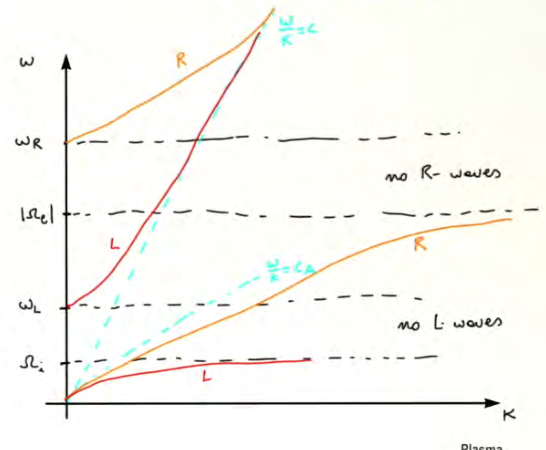
\includegraphics[width=\linewidth]{leftrightfrequencies}

\subsubsection{Whistler waves}

We take the case of R-waves with $\omega / k \ll c \ll \omega_{pe} < \abs{\Omega_e} < \omega_R$ - we're looking at the bottom part of the graph above.

\[(\frac{k c}{\omega})^2 = \frac{(\omega-\omega_R)(\omega+\omega_L)}{(\omega-\abs{\Omega_e})(\omega+\Omega_i)} = \frac{\omega^2 + \omega(\omega_L-\omega_R)-\omega_L\omega_R}{(\omega-\abs{\Omega_e})(\omega+\Omega_i)} \]

This can be simplified by neglecting some terms due to the regime we're in:

\[\frac{k c}{\omega})^2 = \frac{\omega_{pe}^2}{\omega \abs{\Omega_e}} \]

\[ \frac{\omega}{k} = \frac{c}{\omega_{pe}} \sqrt{\abs{\Omega_e} \omega} \]

Functionally this shows that $v_{propagation} \propto \sqrt{\omega}$ and $\pd{\omega}{k} \propto \sqrt{\omega}$ - the propagation (group) velocity increases with frequency. Higher frequency waves propagate faster.

An example - if lightning strikes somewhere on Earth, waves will be produced in the ionosphere and higher frequency ones will propagate faster than slower ones. Here's a neat graph showing that phenomenon:

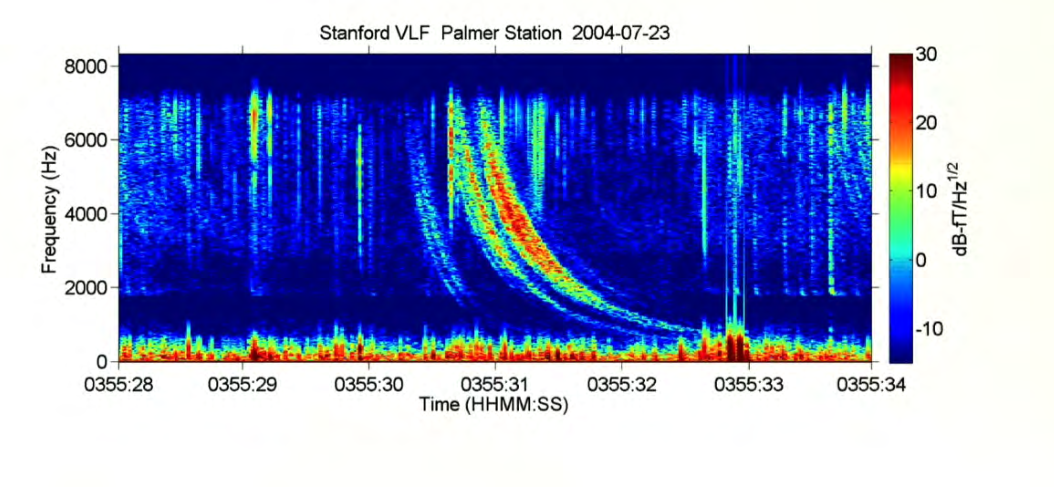
\includegraphics[width=\linewidth]{whistlerwaves}
That actually does sound like whistling! The waves are in the acoustic range!

\subsubsection{Cut-off and resonance frequencies}

For right handed waves:

\[(\frac{k c}{\omega})^2 = \frac{(\omega-\omega_R)(\omega+\omega_L)}{(\omega-\abs{\Omega_e})(\omega+\Omega_i)} \]

$\omega_R$ and $\abs{\Omega_i}$ are frequencies which the waves approach asymptotically. $\omega_R$ is the cutoff frequency: as k goes to 0, $\omega/k$ goes to infinity. k turns from real to imaginary - exponential decay of waves - they don't propagate! Waves are reflected.

Likewise, $\abs{\Omega_i}$ is the resonance frequency: as k goes to infinity, $\omega/k$ goes to zero. Wavelengths decrease, small dissipative processes become important - the wave is absorbed into the plasma.

Of course, for L-waves the cutoff is at $ $ and the resonance is at $ $.



\subsubsection{Properties of waves propagating perpendicular to $B_0$}

For the ordinary mode OM

\[ \omega^2 = \omega_{pe}^2 + k^2 c^2 \]

The cutoff frequency is at $\omega_{pe}$. There's no resonance frequency. As $\omega$ goes to infinity, the propagation velocity approaches c. The limit $\omega$ and $k$ both going to zero cannot be approached by the ordinary mode.

For the extraordinary mode XM

\[ N^2 = \frac{k^2c^2}{\omega^2} = \frac{(\omega^2-\omega_R^2)(\omega^2-\omega_L^2)}{\omega^2-\omega_{LH}^2)(\omega^2-\omega_{UH}^2} \]

Where the lower and upper hybrid frequencies are

\[ \omega^2_{UH} = \Omega_e^2 + \omega_{pe}^2 \]

\[ \omega^2_{LH} = \frac{\Omega_i \abs{\Omega_e} \Big(1+\frac{m_e \Omega_e^2}{m_i\omega_{pe}^2}\Big)}{1+\frac{\Omega_e^2}{\omega_{pe}^2}} \]

There are two cutoff frequencies: $\omega_R$ and $\omega_L$. Likewise, there's two resonances: $\omega_{LH}$ and $\omega_{UH}$. As before, as $\omega$ goes to infinity, the propagation velocity approaches c. As k and $\omega$ approach zero, $\omega = c_A k$ - the Alfven velocity appears!

As before, there's two asymptotes for propagation velocity, this time they're the speed of light and the speed of Alfven:

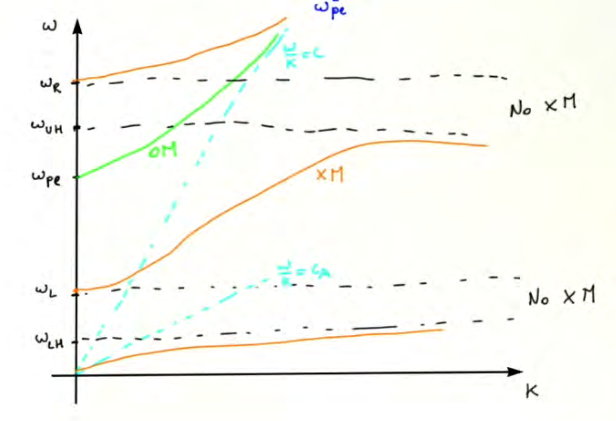
\includegraphics[width=\linewidth]{OMXMfrequencies}

XM waves have two regions where they cannot propagate - between lower hybrid/left and upper hybrid/right hand frequencies.

\end{document}